\documentclass[11pt, letterpaper]{article}
\usepackage[utf8]{inputenc}
\usepackage{graphicx}
\usepackage{indentfirst}
\usepackage{float}
\setlength{\parindent}{5ex}
\renewcommand{\arraystretch}{1.2}

\usepackage{geometry}


\begin{document}

\begin{titlepage}
    \begin{center}
        \vspace*{1cm}

        \Huge
        \textbf{Control Theory \& PID}

        \vspace{0.5cm}
        \LARGE

        \vspace{1.5cm}

        \textbf{Alexander Fogal}

        \vspace{7.8cm}

        \Large
        For Professor Jim Martin\\
        University of Waterloo\\
        August 13th, 2021

    \end{center}
\end{titlepage}

\tableofcontents

\newpage

\section{Introduction}

Hello! This document is meant to be a brief introduction to the topic of Control Theory and specifically PID process control. This document will make constant referecne to PID temperature control, as not only is it a physically intuitive system, but it is also quite important in the real world. 

Essentially, control theory is exactly what it sounds like: a theoretical background for the automatic control of some system (often referred to as a "plant" or "process"). In order to control the system automatically, some sort of feedback is commonly used. A {\it Closed Loop } system is one which measures its own output to determine what input should be used (feedbacking). Sometimes, the terminology {\it Open Loop} will be used as well, this is simply the negation of the closed loop system: there is no feedback control. This usually implies that the input is held constant, although in general one could apply any arbitrary function as input. 

To set the stage: we have some process we wish to control, some means of measuring it, and some input to control it. The goal of a closed loop system is to stabilize the process at some set point by controlling the input in some fashion related to the output of the system. The controllable property of a system is known as the {\it Process Variable} $PV$, which we wish to hold at the set point, $SP$. We can define the error as simply: $e=SP-PV$, and this is the input to our controller, which implements some control function, and outputs the {\it control signal} (control output) $CO=f(e)=f(SP-PV)$. 

For example, say we have some block of metal we wish to hold at a constant temperature. The set point would be the temperature we wish to hold it at, say, $SP=30^{\circ} C$. The process variable here is the measured temperature of the block, which will change over time: $PV=T_{block}(t)$. Then, we have some controller which will take the error in temperature: $e=SP-PV$ and produce the control signal which will control a heater. 

One quick note on terminology, when we write "controller", we mean any arbitrary control process. This may or may not involve a digital controller or a computer, it could even be analogue circuity! For example, tunable lasers are controlled with an analogue feedback loop. For the example of a heater, it is often better to use a digital controller (e.g., a microcontroller like the Arduino), due to the long times involved with heating. 

\section{Control Theory of Feedback Loops}
\subsection{"P" Control}
The most simple form of feedback control is {\it Proportional} control, in which the control signal  is directly proportional to the error term:

$$ CO = k_P e = k_P ( SP-PV) $$

Assuming $k_P>0$ (in the example of a heater, this is generally true, but there may be cause to use a negative value depending on the system!), the control signal is positive when the process variable is below the set point. This makes sense for the heater system: when the temperature of the block (process variable) is below the set temperature (set point), apply some positive work to the heater in order to produce more heat and thereby increase the process variable to the set point. The units of $k_P$ depend on what exactly is meant to be controlled in this situation. We may wish to control a motor, for which the process variable might have units of degrees (aligning a shaft with a set angle), it could be watts for controlling the motor (delivering power to reach a set speed), and in the case of a heater, it could be watts (delivering power to the heater) or even simply amperes (or volts). For the case of the heater, the units of $k_P$ might be $W/^{\circ} C$.

It is rather easy to see the downfalls of such a simple control process, especially for the example system of a heater: when the process variable (temperature) attains the set point, the control signal becomes zero! For a simple argument of why this would not work for a heater, remember that the subject we wish to heat will be radiating heat at all times as well, so we would never reach the set point if the control signal goes to zero as we get close. An easy solution for this is to add a constant term, but the constant term would depend on the material properties of the system, and the whole point was to make less work for ourselves!

\subsection{"PI" Control}
A slightly more sophisticated form of control would be {\it Proportional (and) Integral} control. This involves adding an integral of the error:

$$ CO = k_P \left (e(t) + \frac{1}{T_I} \int_0^t e(\tau) d\tau \right)$$

The addition of the integral term adds a sort of "momentum" or "memory" to the controller. When the process variable is below the set point, the integral term is growing according to the magnitude of the error, and then it will begin to diminish and settle once the process variable exceeds the set point. The integral term may never reach zero though, it will settle to whatever constant value is required by the system to maintain the set point. As for the units of $T_I$, they would be simply the units we are measuring time in. A physical intuition for $T_I$ (often called the repeat time or integration time) is that it is the amount of time required for the integral term to match the contribution of the proportional term.

For heater control, this is really all that is needed, but it is not too hard to imagine a system where overshooting the set point is unacceptable, or where we cannot afford to wait for the system to settle after reaching the set point. So how do we manage this?

\subsection{"PID" Control}
The "fully featured" control paradigm: {\it Proportional, Integral, Derivative} control. Very powerful and very robust, this paradigm can be used to control all matter of processes. As the name suggests:

$$ CO =  k_P \left( e(t) + \frac{1}{T_I} \int_0^t e(\tau) d\tau + T_D \frac{de}{dt} \right)$$

The addition of the derivative term allows the controller to know how fast the process variable is tending toward the set point and adjust accordingly in order to not overshoot. This would be useful say, for the case of a motor that must turn to a specific angle and no further. The constant $T_D$ is also in units of time. 

\subsection{Properties of PID}
As a quick note, one can pick and choose any of the three PID terms to control the process. As mentioned previously, PI control is sufficient for the case of a heater system. 
\\ \\
One must be careful with their choice of coefficients for PID control though, as PID is a feedback algorithm, it is susceptible to things like feedback loops and oscillation (think mic into an amplified speaker feedbacking). In our heater example, the heat takes time to go from the heater to the thermistor being used to measure and provide feedback. This may not sound like a big problem, but it creates the opportunity for disturbances to build into feedback loops. The phase lag incurred as the heat wave travels from the heater is frequency dependant, and due to the integration term, the system will not settle right away. At low frequencies, the process variable tracks with the control signal, but at higher frequencies, significant phase lag is incurred, resulting in maximum control signal occurring in tandem with maximum change in the process variable and so the process variable will oscillate and not come to equilibrium.

The ratio of the control signal to the process variable amplitude (often expressed as a function of frequency) is referred to as the {\it loop gain} of the process. If we were using only P control, the loop gain would be constant and equal to $k_P$. Under PI control, the gain goes to infinity as frequency goes to zero. The gain is unitless, as the units of the process variable are the inverse of the units of the control signal. This product, often expressed in complex form as a function of frequency, is called the {\it transfer function} of the system. We can model and then analyze this equation in order to mathematically guarantee the stability of our system and the robustness of the control.

\section{Modelling and Analyzing PI Heater Control}
As mentioned in the previous section, we wish to model and analyze the transfer function of the system (the product of the control equation and the process equation) in order to guarantee the stability of our system. 

\subsection{A Quick Aside on the Laplace Transform}
The Laplace transform comes up a lot in Control Theory, it appears when describing linear time invariant systems and the definition of transfer functions. Linear systems are linear in the sense that: $c_1 f(a)+c_2 f(b) = f(c_1 a + c_2 b)$ (in practise this implies that the process transfer function is not dependant on operating point, and behaves the same everywhere), time invariant systems are systems where the output does not depend on when an input was applied (i.e. we can set $t=0$ and do time shifts arbitrarily). For example, most electrical circuits can be approximated by linear and time invariant models. The intuition and physical reasoning for using the Laplace transform in this case is quite hard to appreciate. One can think of the Laplace transform as arising from the idea of impulse responses of the system, or even just that it is convenient for learning properties of the system. For example, the function space that is the output of the Laplace transform allows us to define a norm, and therefore a notion of "closeness" between transfer functions. This is useful to define the robustness of a system: a control scheme that works not just for the subject model, but for "nearby" models as well, can be considered robust. 

Whether one chooses to think of the Laplace transform as a convenient piece of mathematics or as a physically meaningful process, it cannot be ignored in the analysis of systems, particularly since many systems can be approximated as linear and time invariant, and perturbation analyses on these systems are useful as well. To at least convince the reader of its usefulness, any linear and time invariant system can be expressed as:

$$ y(t) = \int_{-\infty}^{\infty} h(t-\tau)u(\tau)d\tau $$

For which the Laplace transform is:

$$ Y(s) = H(s)U(s) $$

simply multiplication. The function $h(t)$ being the impulse response, $H(s)$ being the transfer function, $u(t)$ being the input to the control, $y(t)$ being the output of the control. That is to say, the system is entirely characterized by either the transfer function or the impulse response. We also generally take $s=i\omega$ ($\omega$ being frequency), so the transfer function is a function of frequency only. For more see Olivi, Martine in the reference section.


I will also quickly note that the Z transform is equivalent to the Laplace transform acting on discrete time systems.

\subsection{Modelling PID Control}
The transfer function of the PID control scheme is achieved by taking the Laplace transform of the control signal equation:

$$ H(s) = k_P \left( 1 + \frac{1}{T_I s} + T_d s \right) = k_P \left( 1 + \frac{1}{i \omega T_I } + i \omega T_D  \right) $$

From here on, we will take $T_D = 0$ (PI control only). Our model is therefore: 

$$ H(\omega) = k_P + \frac{k_P}{i\omega T_I} $$

Where the constants are as defined in the PID control scheme.

\subsection{Modelling a Heater System}
Our model for the heater system will consist of two parts: a first order lag, modelled by a low pass RC filter (first term), and a time delay modelled simply by a phase lag (second term). Altogether, this gives us:

$$ G(\omega) = \frac{K}{1+i\omega T_{1}} e^{-i \omega T_d} $$

The constant $K$ (not to be confused with $k_P$) is the loop gain, $T_1$ is first order time lag, and $T_d$ is the time delay. The time delay models the time it takes the heat wave to travel from the heater to the thermistor making the measurements, and the low pass filter models the properties of heat in a medium. 

\subsection{System Model and Stability}
The full model transfer function of our system is now:

$$ H(\omega)G(\omega) = \left( k_P + \frac{k_P}{i \omega T_I}\right)\left( \frac{K}{1+i\omega T_{1}} e^{-i \omega T_d} \right)$$

Now, we can begin to assess the stability of this system using the Nyquist Criterion. Essentially, the Nyquist criterion states that, in order for a system to be stable, it must have a gain of less than unity at a phase of $180^{\circ}$ (and odd multiples, e.g. $540^{\circ},900^{\circ},$ etc.). Graphically, that means that the function must not encircle the point $-1+0i$ in the complex plane. There is more discussion of the related mathematics in Wescott, Tim.

Only one problem, the coefficients in the model are undetermined! For this we have the Ziegler-Nichols design approach.

\subsubsection{Fitting the Heater Model and Determining PID Coefficients}
Essentially, fitting the model is accomplished via graphical construction, but first, we need data. The data in question is called the {\it open loop step response} of the process. This involves setting the input to the process to a constant value, waiting for the process variable to settle, and then increasing the input to some higher value and waiting for it to settle once more. The graph will ideally look like this:

\begin{figure}[H]
    \centering
    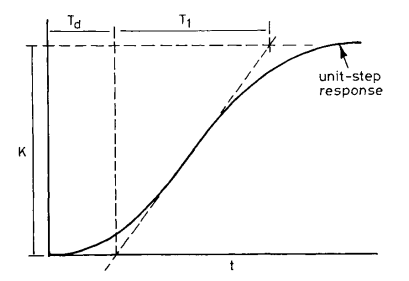
\includegraphics[width=8cm]{openLoopStep.png}
    \caption{ Showing how the coefficients of the model may be determined from step response. Note that it is not important that it be a unit step response, appropriate scaling may be applied instead. }
    \label{fig:openLoopStep}
\end{figure}

In reality, it can be quite a bit messier:

\begin{figure}[H]
    \centering
    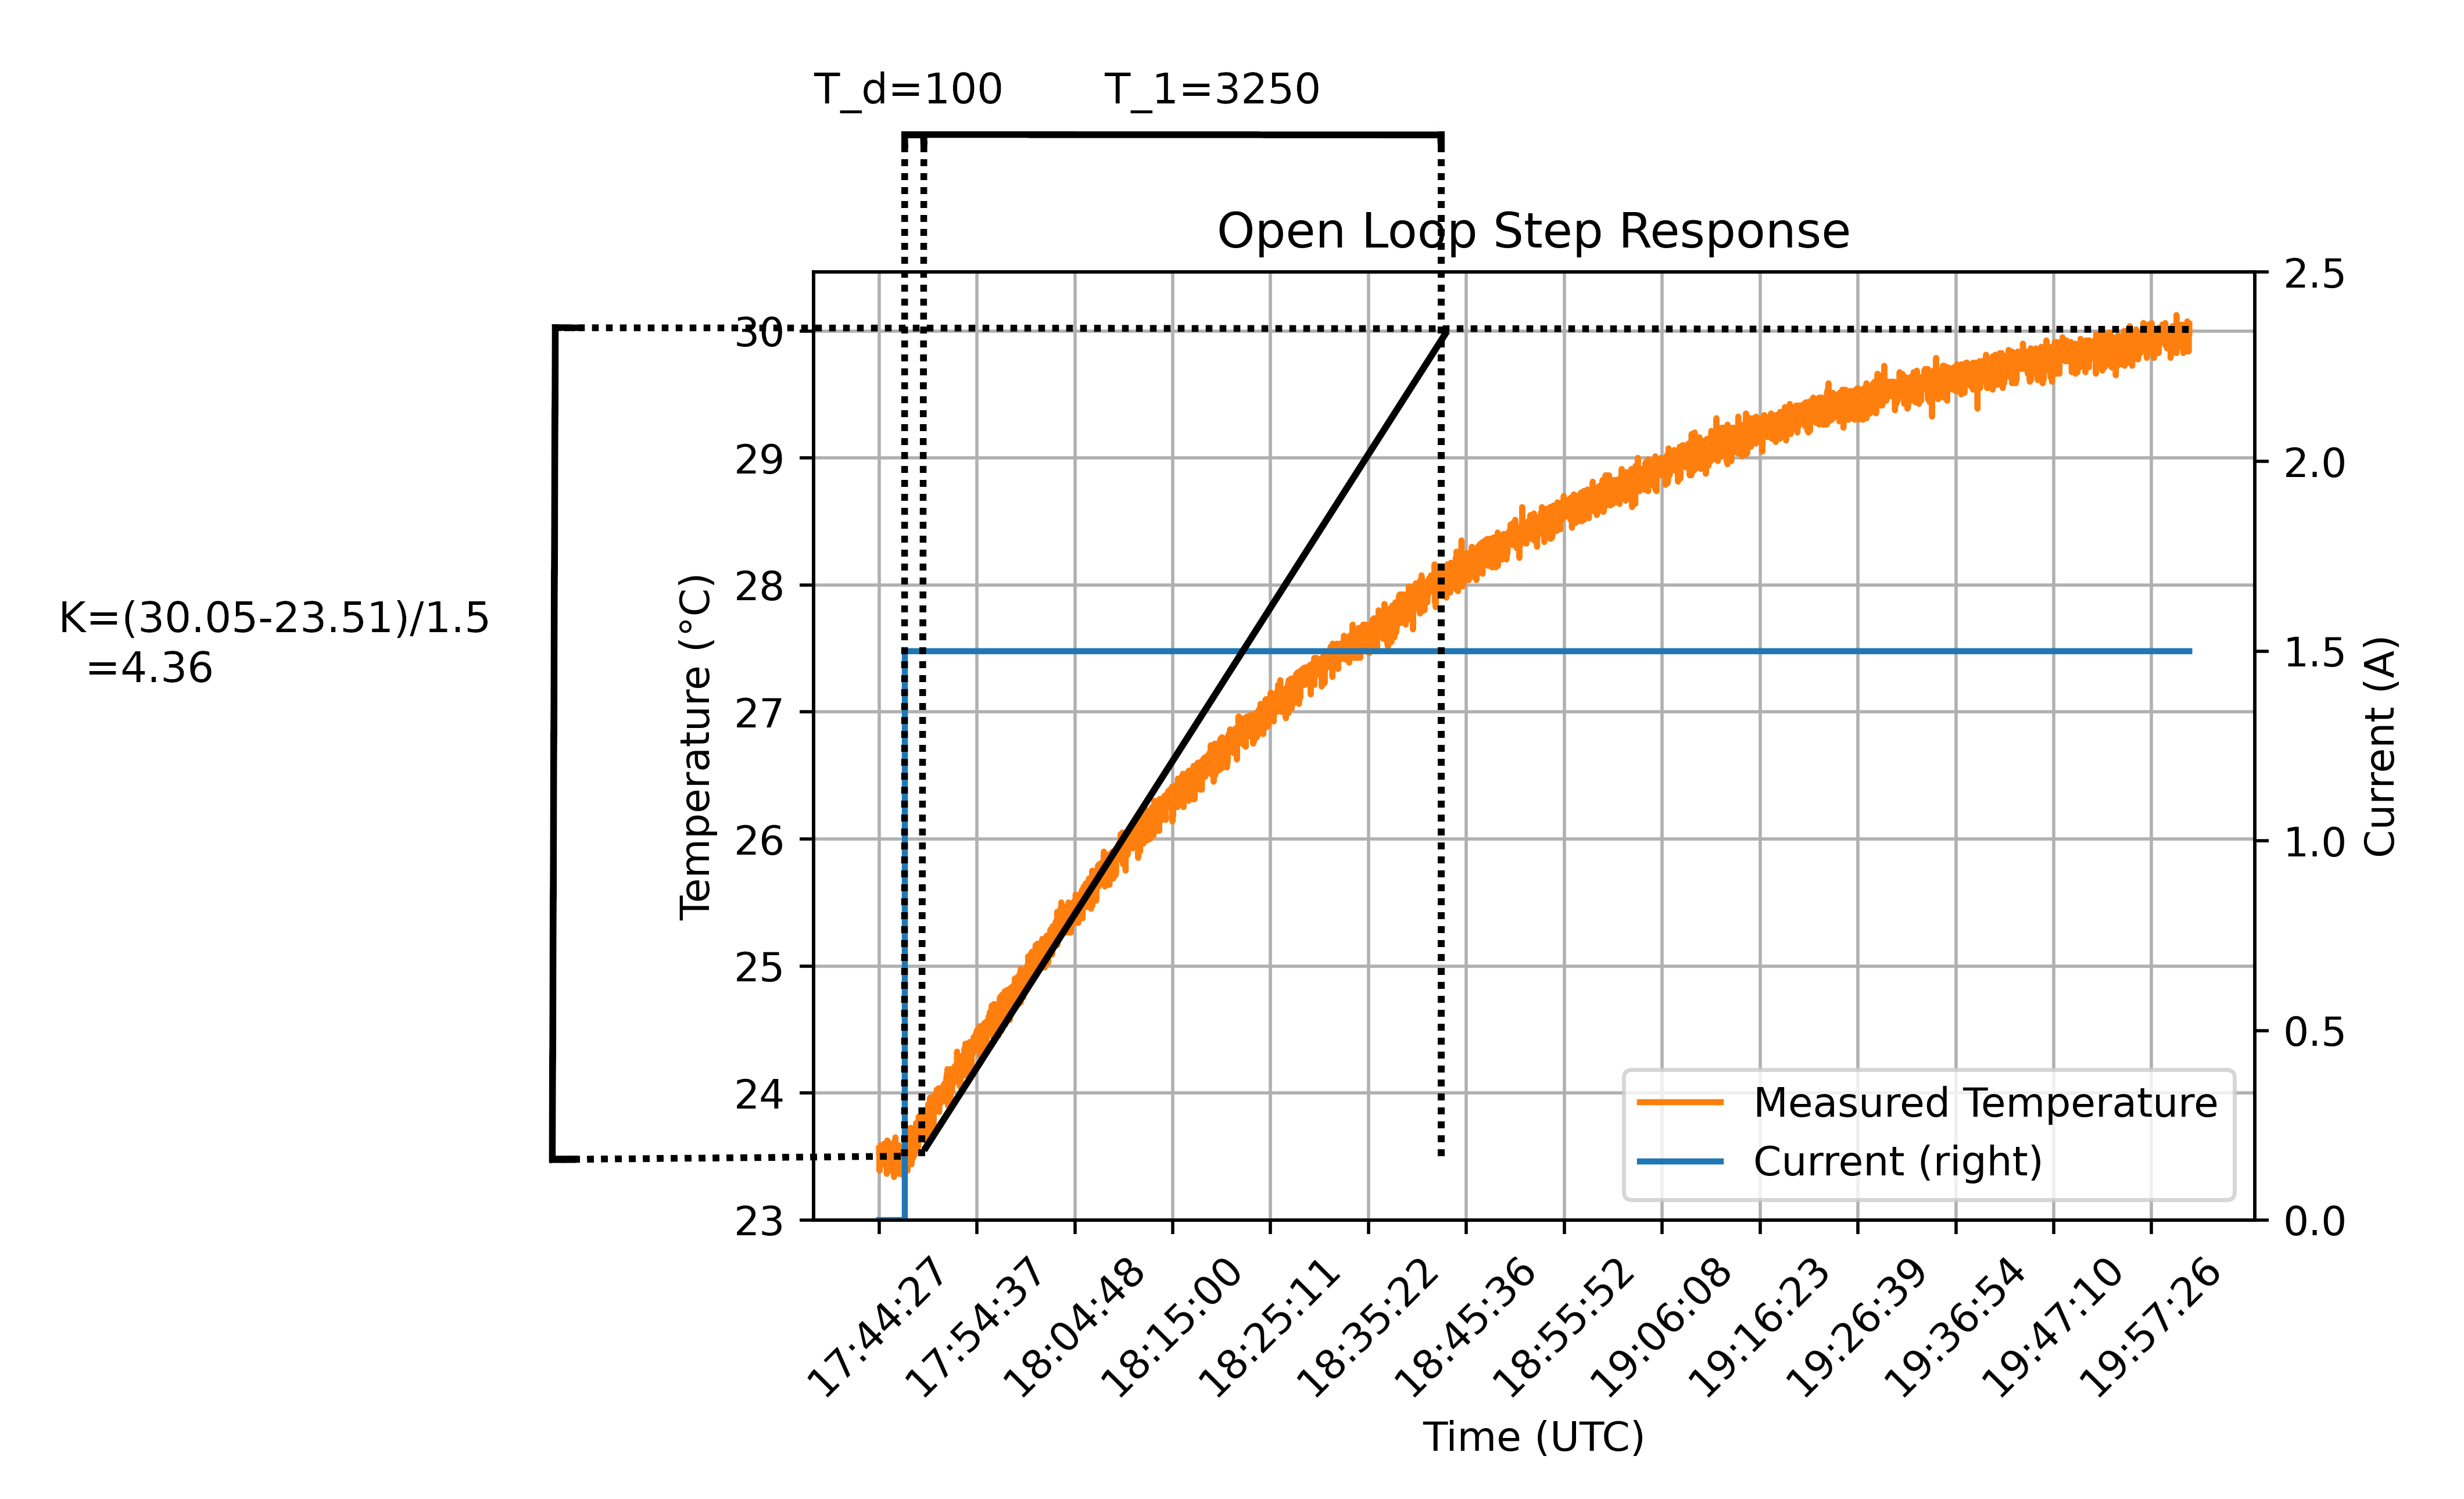
\includegraphics[width=18cm]{realOpenLoopStep.png}
    \caption{ Actually determining coefficients from data. Note that it is verging on impossible to directly use the graph, and digging through the data points will almost certainly be necessary. }
    \label{fig:realOpenLoopStep}
\end{figure}

Given the above values extracted from the data, the following PID coefficients are recommended for stability and optimal control:

\begin{table}[H]
\centering
\begin{tabular}{llll}
     & $k_P$ & $T_I$ & $T_D$  \\[0.3cm] \hline
 P   & $\frac{T_1}{kT_d}$  & -  & - \\[0.3cm]
 PI  & $\frac{0.9 T_1}{KT_d}$  & $3.3T_d$ &  -\\[0.3cm]
 PID & $\frac{1.2 T_1}{KT_d}$  & $2T_d$  & $0.5T_d$
\end{tabular}
\end{table}

\subsubsection{Assessing Stability}
Now that all the coefficients are determined, we can plot the transfer function as a function of frequency in the complex plane. The easiest way to do this is to expand the complex exponentials as a sum of cosines and sines, collect into the form $a(\omega)+ib(\omega)$ and then plot it as a parametric curve, $(a(\omega),b(\omega))$. Having done that gets the following:

\begin{figure}[H]
    \centering
    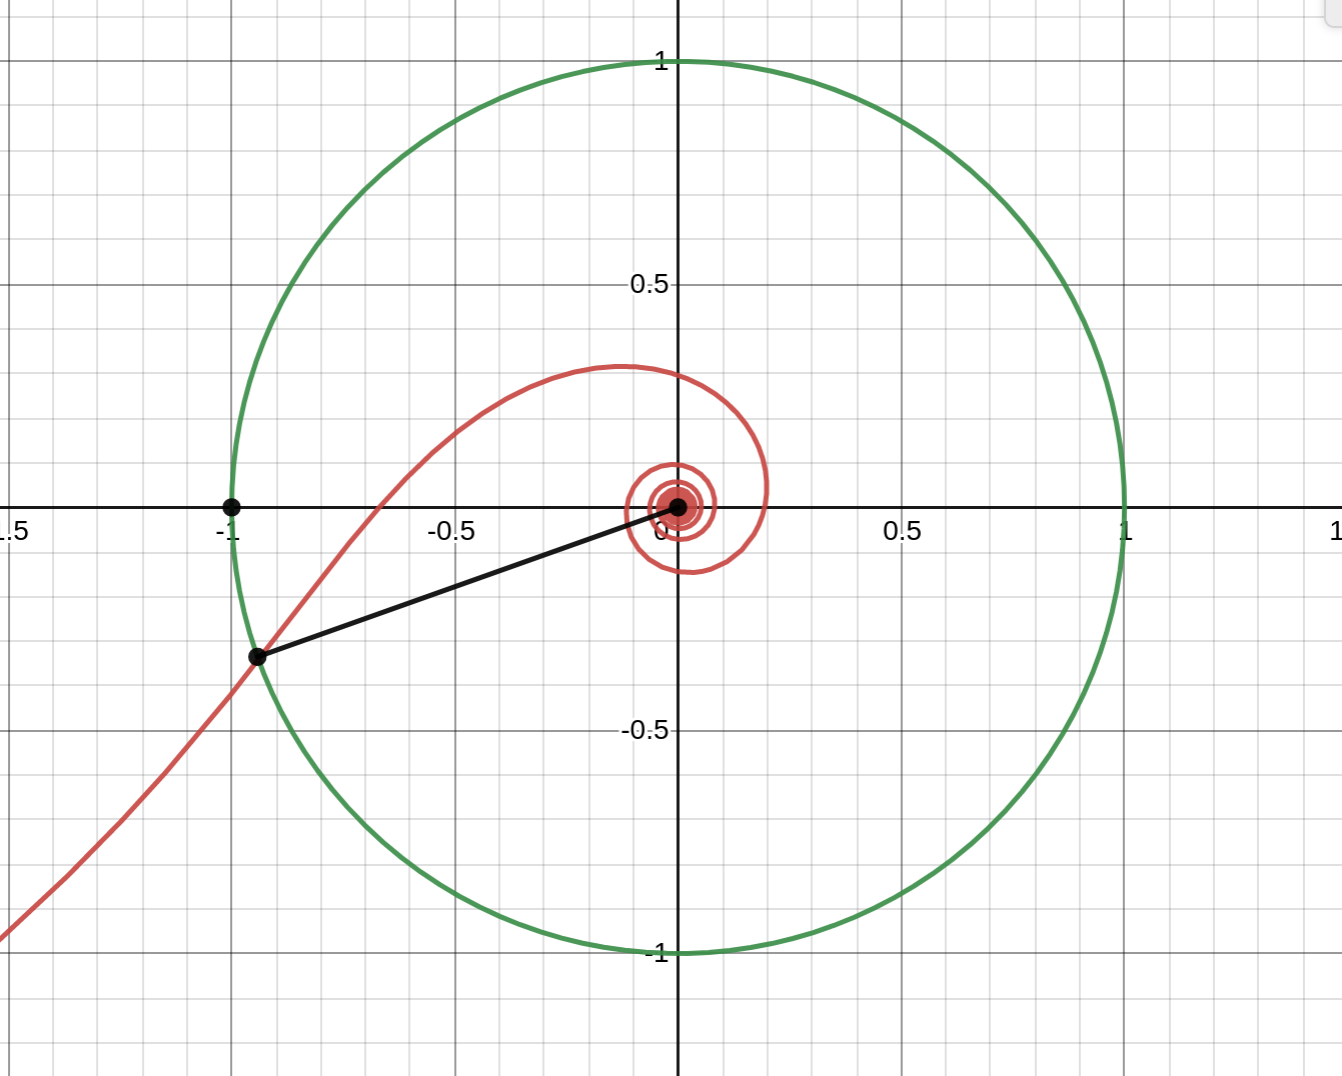
\includegraphics[width=12cm]{nyquistPlot.png}
    \caption{ A plot showing the function as a parametric curve over frequencies $\omega=0...10$ and a unit circle. Note that the curve tends to $-\infty$ on the $y$ axis, which corresponds to the integral having infinite gain (an integrator always contributing a phase of $90^{\circ}$) at zero frequency. Note that the curve does not encircle $-1+0i$ as required for stability. The gain margin here is $3.5$dB and the phase margin is $20^{\circ}$. }
    \label{fig:nyquistPlot}
\end{figure}

There are two factors involved with assessing the stability in relation to the Nyquist criterion: gain margin and phase margin. The gain margin (in dB) is a notion of how far away from oscillation the system will be when the frequency is such that the phase lag is exactly $180^{\circ}$, which is expressed as:

$$ g = 20 \log_{10} \left( -Re(H(\omega^*))\right) $$

In order to assess gain margin, we must first find the frequency corresponding to the closest root to the point $-1+0i$ and then plug that frequency, $\omega^*$, into the real part of the transfer function, and then apply the rest of the above formula.

The phase margin is the angle between the $-x$ axis and the point at which the function intersects the unit circle. In other words, it is the difference in phase between the critical point and where the function is magnitude unity (remember that the function must have less than unity gain at phase $180^{\circ}$). In order to assess phase margin, one must first find the frequency at which the magnitude of the transfer function is 1, i.e., $|H(\omega^*)|=1$ (please excuse my abuse of notation from reusing $\omega^*$ for this, they are not otherwise related).  After that, the transfer function should be put in the form $|H|e^{i\phi}$, and then the phase margin will be $180^{\circ} - \phi$. 

\section{In Practise}
If we have done everything up until now correctly, we will expect that the controller will do a few easily identifiable things. First, when we set the set temperature, the measured temperature should approach and overshoot this, and then exhibit first order decay until settling on the set temperature. Second, this should result in some approximately constant (over short periods of time, since over long periods of time the ambient temperature and therefore the level of current required to maintain a certain temperature, will change) amount of current being delivered.

The closed step response should therefore look like this:

\begin{figure}[H]
    \centering
    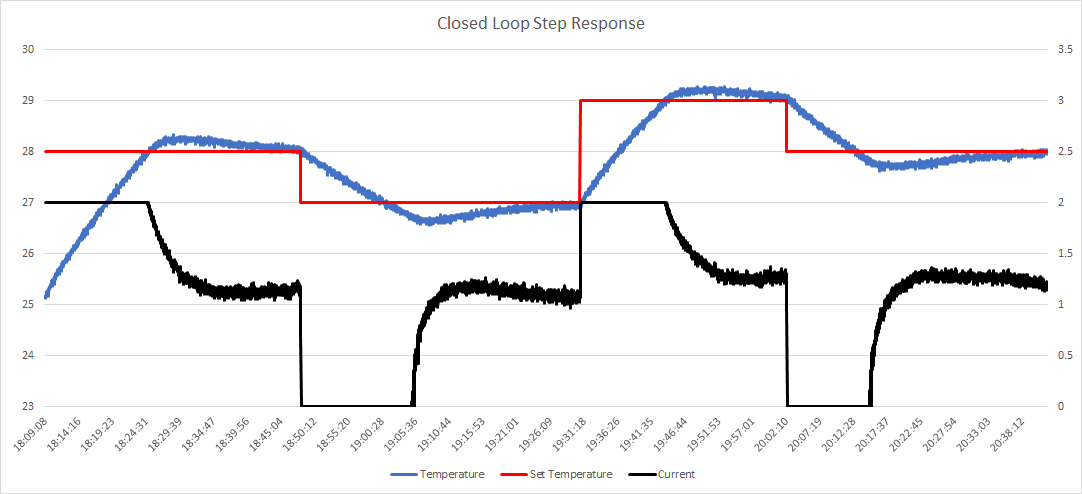
\includegraphics[width=16cm]{closedLoopStep.png}
    \caption{ Forgive my not labelling the axes, the left axis is temperature in Celsius, and the right is current in amperes. The bottom axis is time in UTC. }
    \label{fig:closedLoopStep}
\end{figure}

\newpage
\section{References and Further Reading}
\begin{enumerate}
    \item Jones, Lucas: Practical Implementation of Temperature Control
    \item Martin, James: Notes on Feedback and Oscillations
    \item Olivi, Martine: The Laplace transform in control theory \\ https://www-sop.inria.fr/apics/sbpi/LtransformOlivi.pdf
    \item Forgan, E.M.: On the use of temperature controllers in cryogenics \\ https://doi.org/10.1016/0011-2275(74)90190-8
    \item Wescott, Tim: Applied Control Theory for Embedded Systems
\end{enumerate}

\end{document}